% !Mode:: "TeX:UTF-8"
\documentclass{beamer}

\mode<presentation>
{
\usetheme{Warsaw}

\setbeamercovered{transparent}
}

\usepackage[UTF8]{ctex} % 支持中文

% 分页Slide不编号
\setbeamertemplate{frametitle continuation}{}

% 插入多列
\usepackage{multicol}

% 插入链接
\usepackage{hyperref}
\hypersetup{urlcolor=blue}

% 插入图片
\usepackage{graphicx}

% 插入代码
\usepackage{xcolor}
\definecolor{mygray}{RGB}{245,245,245}

\usepackage{listings}
\lstset{language=Python}
\lstset{escapeinside=``}
\lstset{numbers=left}
\lstset{breaklines}
\lstset{backgroundcolor=\color{mygray}}

% 书签乱码解决方案
% 在文件D:/CTEX/MiKTeX/tex/latex/beamer/base/beamer.cls 中找到:
% \PassOptionsToPackage{bookmarks=true,%
%   bookmarksopen=true,%
%   pdfborder={0 0 0},%
%   pdfhighlight={/N},%
%   unicode=true,%       <-------------- 加入此行
%   linkbordercolor={.5 .5 .5}}{hyperref}

% If you have a file called "university-logo-filename.xxx", where xxx
% is a graphic format that can be processed by latex or pdflatex,
% resp., then you can add a logo as follows:

% \pgfdeclareimage[height=0.5cm]{university-logo}{university-logo-filename}
% \logo{\pgfuseimage{university-logo}}



% Delete this, if you do not want the table of contents to pop up at
% the beginning of each subsection:
\AtBeginSubsection[]
{
\begin{frame}<beamer>
\frametitle{目录}
\begin{multicols}{2}
\tableofcontents[currentsection,currentsubsection]
\end{multicols}
\end{frame}
}

% If you wish to uncover everything in a step-wise fashion, uncomment
% the following command:

%\beamerdefaultoverlayspecification{<+->}

\begin{document}

\title{项目简介-数据组}

% - Use the \inst{?} command only if the authors have different
%   affiliation.
%\author{F.~Author\inst{1} \and S.~Another\inst{2}}
\author{张祎璘}

% - Use the \inst command only if there are several affiliations.
% - Keep it simple, no one is interested in your street address.
\institute[Universities of]
{
厦门大学\quad 经济学院}

\renewcommand{\today}{\number\year 年 \number\month 月 \number\day 日}
\date{\today}

% This is only inserted into the PDF information catalog. Can be left
% out.
\subject{Presentations}

% title page
\begin{frame}
\titlepage
\end{frame}

% content
\begin{frame}
\frametitle{目录}
%\begin{multicols}{2}
\tableofcontents%[currentsection,currentsubsection]
%\end{multicols}
% You might wish to add the option [pausesections]
\end{frame}

\section{CPI结果与分析}
\subsection{CPI简介与总指数}
\begin{frame}
\frametitle{CPI结果与分析}
官方CPI的的计算将商品分为八大类,分别是食品,烟酒,服装,家庭设备,医疗保健,交通通信,教育娱乐,居住。

八个大类又依次分为中类,小类和基本分类。

反映的是价格的变动状况,也可以理解为今天所有商品均价除以上一天得到的一个指数。
\end{frame}
\begin{frame}
\frametitle{CPI结果与分析}
价格指数结果:
\begin{itemize}
  \item 价格指数基本大于一,反映通货膨胀。
  \item 双十一的价格急剧下降
  \item 第二天价格指数并未出现剧烈上升,部分商品在双十一过后折扣仍然存在
\end{itemize}
\end{frame}
\begin{frame}
\frametitle{CPI结果与分析}
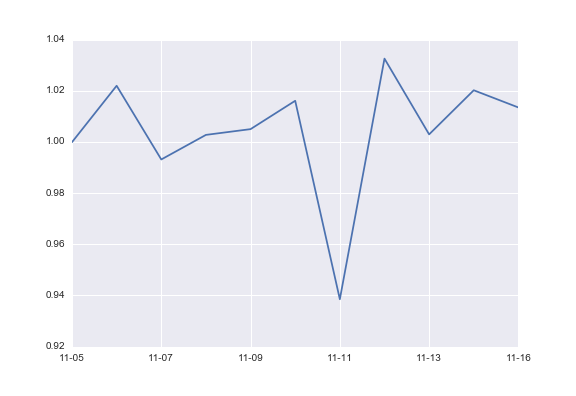
\includegraphics[width=10cm,height=7cm]{double11_totalindex.png}
\end{frame}

\subsection{大类指数}
\begin{frame}
\frametitle{CPI结果与分析}
八个大类的价格指数:
\begin{itemize}
  \item 整体和总的价格指数波动相近,存在部分的差异
  \item 衣服的价格下降最为剧烈,其次是医疗产品,交通和通信产品
  \item 烟酒的价格指数有待进一步探讨
\end{itemize}
\end{frame}
\begin{frame}
\frametitle{CPI结果与分析}
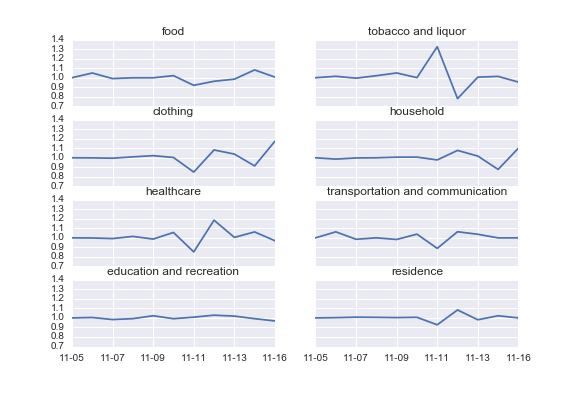
\includegraphics[width=10cm,height=7cm]{double11_8cate.png}
\end{frame}

\subsection{服装指数}
\begin{frame}
\frametitle{CPI结果与分析}
服装中的小类价格变化:
\begin{itemize}
  \item 女装的价格下降最明显,其次是男装,然后是儿童
\end{itemize}
\end{frame}
\section{}
\subsection{}
\begin{frame}
\frametitle{CPI结果与分析}
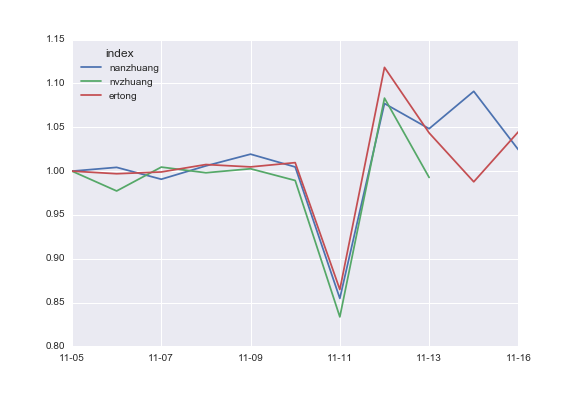
\includegraphics[width=10cm,height=7cm]{double11_data_addindex.png}
\end{frame}


\section{价格描述}
\subsection{总体价格变动分布}
\begin{frame}
\frametitle{价格描述}
价格变动大小统计描述:
\begin{itemize}
  \item 双十一价格平均下调8\%
  \item 最大折扣为90.5\%
  \item 43.3\%的商品价格相对于10号没有变动
  \item 55.0\%的商品价格相对于10号下降
  \item 1.7\%的商品价格相对于10号上涨
\end{itemize}
\end{frame}
\begin{frame}
\frametitle{价格描述}
双十一之后的十二号的价格变动:
\begin{itemize}
  \item 十二号价格相对于十号价格打折1\%,部分商品保持双十一的价格,折扣延续
  \item 87.7\%的价格在十二号回调至十号的价格
  \item 9.0\%的价格在十二号仍然保持十一号大减价的状态
\end{itemize}
\end{frame}
\begin{frame}
\frametitle{价格描述}
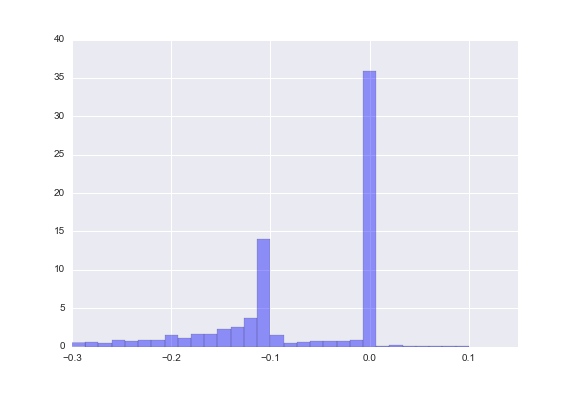
\includegraphics[width=10cm,height=7cm]{all_pr.png}
\end{frame}

\subsection{食品和衣着价格变动分布}
\begin{frame}
\frametitle{价格描述}
食品价格变动:
\begin{itemize}
  \item 食品在双十一整体折扣幅度为7.4\%,比总体的8%略低
  \item 双十一最高折扣为88.8\%
  \item 双十一食品中,50.8\%的价格下降,46.5\%的价格保持不变
  \item 十二号,8.4\%的商品继续保持双十一打折的状态,87.7\%的商品回调至十号的价格
\end{itemize}
\end{frame}
\begin{frame}
\frametitle{价格描述}
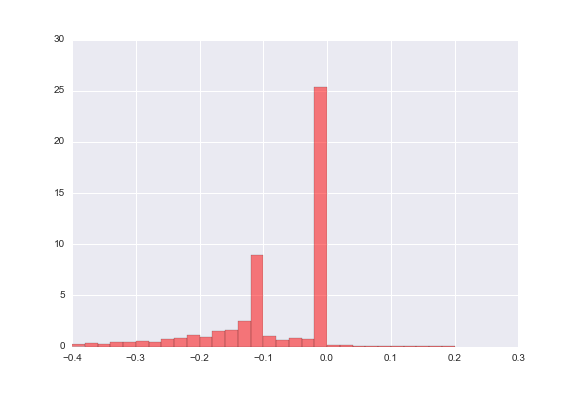
\includegraphics[width=10cm,height=7cm]{cate1_pr.png}
\end{frame}
\begin{frame}
衣着的价格变化状况。
\frametitle{价格描述}
\begin{itemize}
  \item 衣着在双十一整体折扣幅度为15.8\%,基本是总体的8\%的两倍
  \item 双十一最高折扣为82.1\%
  \item 双十一衣着中,90.9\%的价格下降,8.9\%的价格保持不变
  \item 十二号,14.1\%的商品继续保持双十一打折的状态,83.6\%的商品回调至十号的价格
\end{itemize}
\end{frame}
\begin{frame}
\frametitle{价格描述}
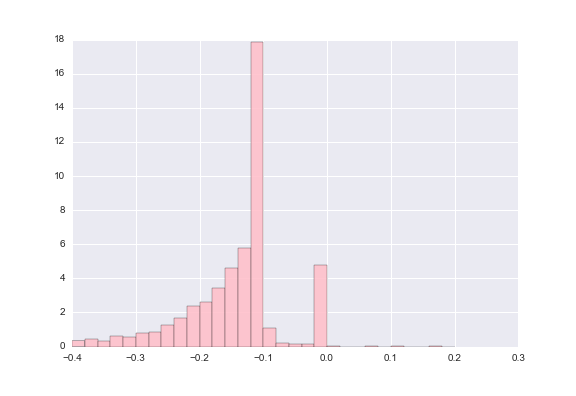
\includegraphics[width=10cm,height=7cm]{cate3_pr.png}
\end{frame}


\section{销量变化}
\subsection{总体销量变化}
\begin{frame}
\frametitle{销量变化}
我们对销量加1取log值,再用本天减去上一天的销量,来表现每天的销量变化
\begin{itemize}
  \item 官方更新销量数据是有延迟的,11-13的数据实际上反映的是11-11的销售量。
  \item 11-11和11-12的销量出现非常大的增加,平台活动刺激了消费
  \item 11-11和11-12前后的销量都比上月少,平台活动日抑制了活动日前后的消费
\end{itemize}
\end{frame}
\begin{frame}
\frametitle{销量变化}
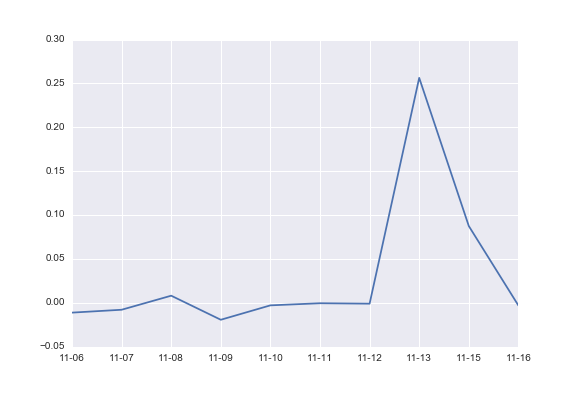
\includegraphics[width=10cm,height=7cm]{double11_data_bigquatity.png}
\end{frame}

\subsection{大类销量变化}
\begin{frame}
\frametitle{销量变化}
下面我们来看八个大类的销量变化
\begin{itemize}
  \item 增加最多的是衣服,教育娱乐产品
\end{itemize}
\end{frame}
\begin{frame}
\frametitle{销量变化}
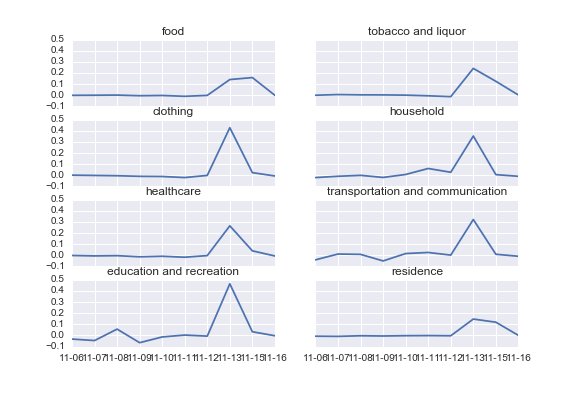
\includegraphics[width=10cm,height=7cm]{double11_data_totalquatity.png}
\end{frame}


\begin{frame}
\begin{center}
  
\includegraphics[width=7cm,height=7cm]{CPP.jpg}
\end{center}
\end{frame}

\end{document}
